\chapter{Result Analysis and Testing}\label{chap4}



\vspace*{40 ex}
%============================================================
\paragraph*{Outline:} This chapter presents the following:
\begin{enumerate}
\setlength{\itemsep}{-0.3em}
\item Introduction
\item Source Code
\item Result Analysis 
\item Test Cases
\end{enumerate}
%============================================================

\newpage

\section{Introduction}\label{chap4:intro}
After study of existing system,software requirements,system analysis and Implementation let us have a look optimum source code acceptable results analysis and their possible test cases.

\section{Source Code}

\subsection{Screenshot}

\begin{figure}[!ht]
	\centering
	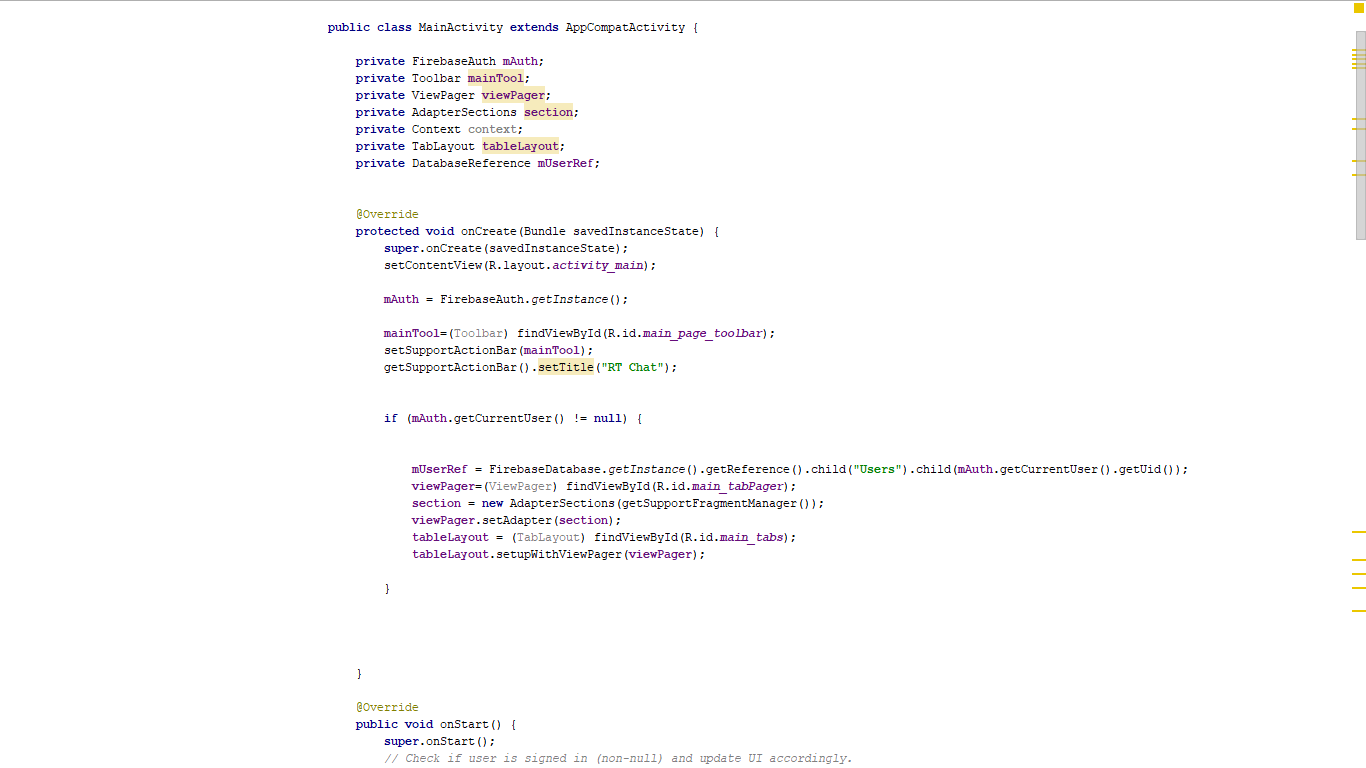
\includegraphics[scale=0.2]{main.png}
	\caption{\label{img11} Home page activity code which contains all home fragments }
\end{figure}

\noindent
\begin{figure}[!ht]
	\centering
	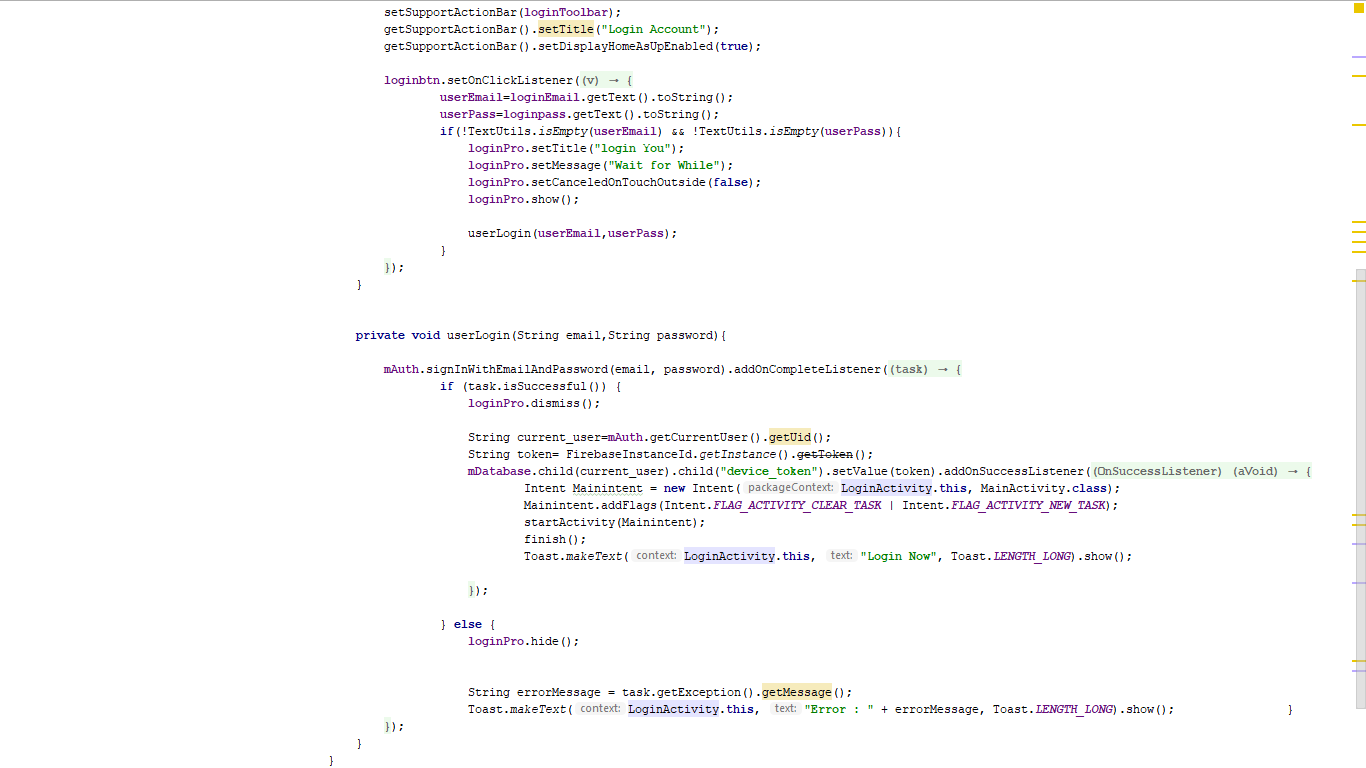
\includegraphics[scale=0.3]{login.png}
	\caption{\label{img12} Login activity code where user will login }
\end{figure}

\noindent
\begin{figure}[!ht]
	\centering
	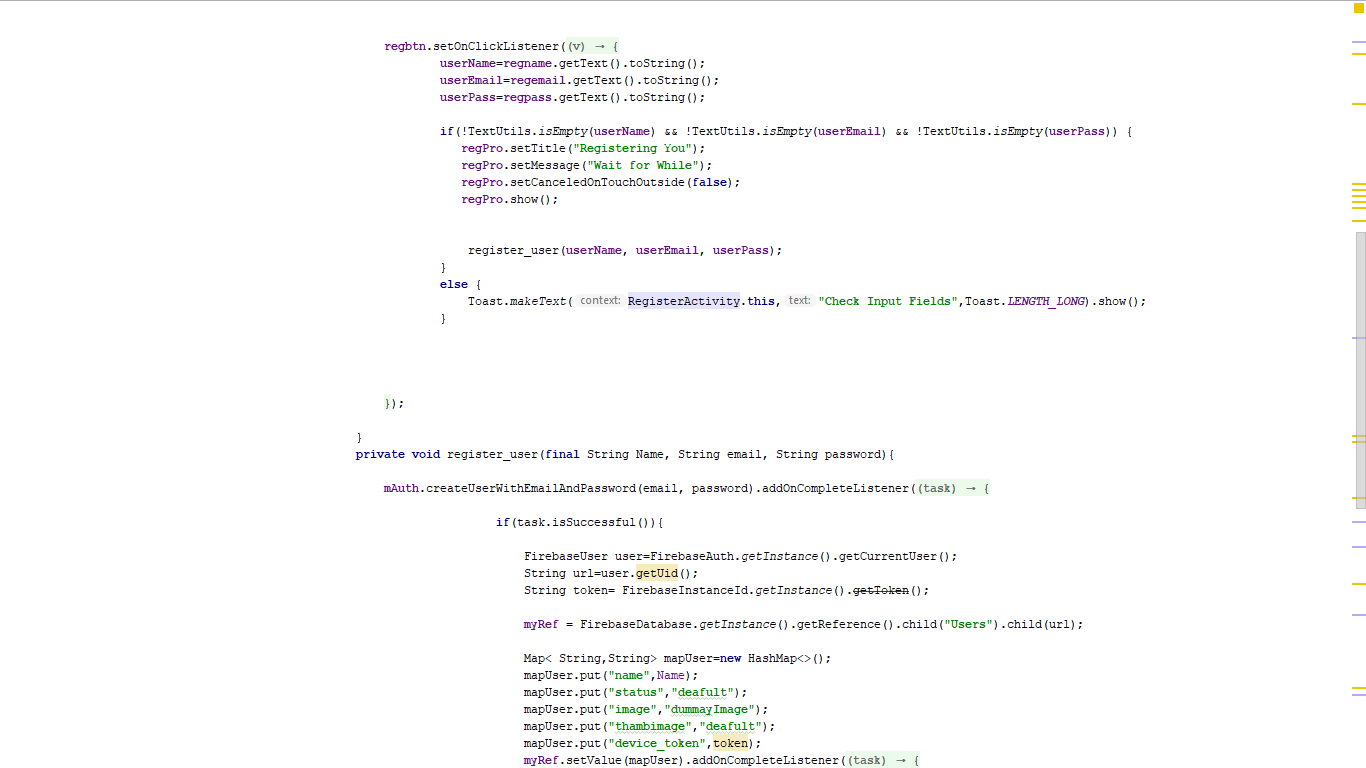
\includegraphics[scale=0.3]{register.png}
	\caption{\label{img13} Register activity code where user will register}
\end{figure}

\noindent
\begin{figure}[!ht]
	\centering
	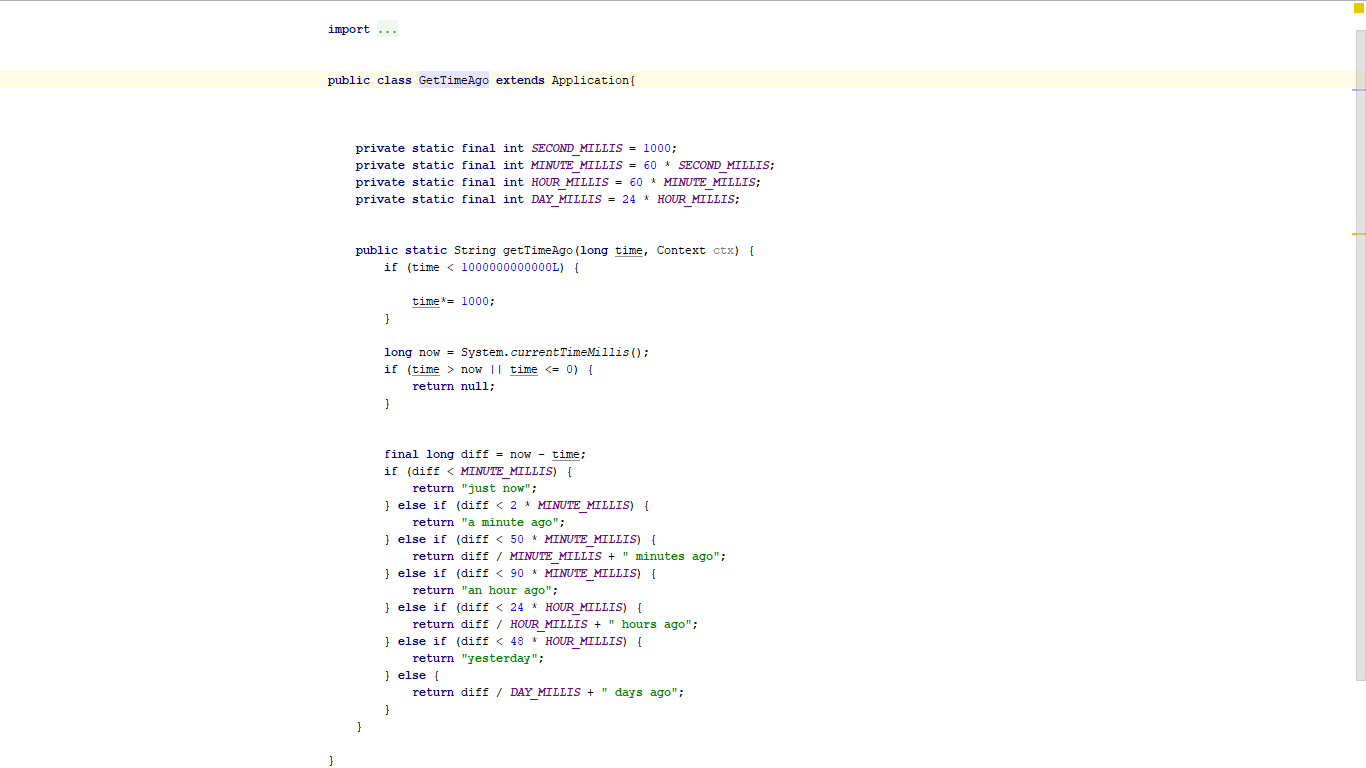
\includegraphics[scale=0.3]{time-convert.png}
	\caption{\label{img14} Script to convert firebase timestamp to real time }
\end{figure}

\noindent
\section{Result Analysis}
From a proper analysis of positive points and constraints on the component, it can be safely concluded that the product is a highly efficient GUI based component. This application is working properly and meeting to all user requirements. This component can be easily plugged in many other systems.

\subsection{Application Objectives :- }

\begin{enumerate}
	\setlength{\itemsep}{-0.3em}
	\item  \textbf{Improvement in control and performance :}\\ The system is developed to cope up with the current issues and problems with all needed thing are situated to different-different places.
	\item  \textbf{Save cost :}\\ After computerized application is implemented less human force will be required to maintain user information like messages, blog post and most important popular news thus reducing the overall cost.\\
	\item \textbf{Save time :}\\ User is able to search popular news by using few clicks on screen and few search keywords thus saving his valuable time\\
	\item \textbf{Save effort :}\\ In current time people has no such time to cope-up with all possible thing to go at all possible places so that all thing regarding current popular news,messages chat, blog post will come at my proposed project. 
\end{enumerate}


\section{Test Cases}
The aim of the application testing process was to determine all defects in our project .The program was subjected to a set of test inputs and various observations were made and based on these observations it will be decided whether the program behaves as expected or not

\bigskip
\noindent
Items to be tested :-  
\begin{enumerate}
	\item create Account
	\item Login in Account
	\item Home Page
	\item Home Page Fragments
	\item User Profile
	\item Chatting feature
	\item Chat messages status
	\item Blog Post
	\item Like and Comments
	\item All user or Find friends
	\item User Status
	\item User Online and Offline Status 
	\item Recent Popular News
	\item Specific News
	\item Share News
	\item News open with browser
	
\end{enumerate}

\subsection{Test for Home Page Activity}
There is following scenario come over user home page activity...
\begin{itemize}
	\item When user gets login or register then user will come this home page activity
	\item This home page activity contains four fragments and one menu bar.
	\item Fragment CHATS contains list of all the chats with user friends and if user clicks any of his friend he or she will go to his chat list with friend. 
	\item Fragment FRIENDS contains list of user friends and if user clicks any of his friend then he or she will find two options first chats and second their profile.
	\item Fragment REQUESTS contains list of friend request and their type sent or received and if user clicks any of them form list then he or she will go to their profile .
	\item When user clicks on POST fragment then he or she will be reached at blog post page.
	\item Menu Bar contains five things..
	\begin{enumerate}
		\setlength{\itemsep}{-0.3em}
		\item All Users Post
		\item Popular News
		\item All Users List or Find Friends.
		\item User account setting
		\item Logout
	\end{enumerate}
	    
\end{itemize}
\noindent
\begin{figure}[!ht]
	\centering
	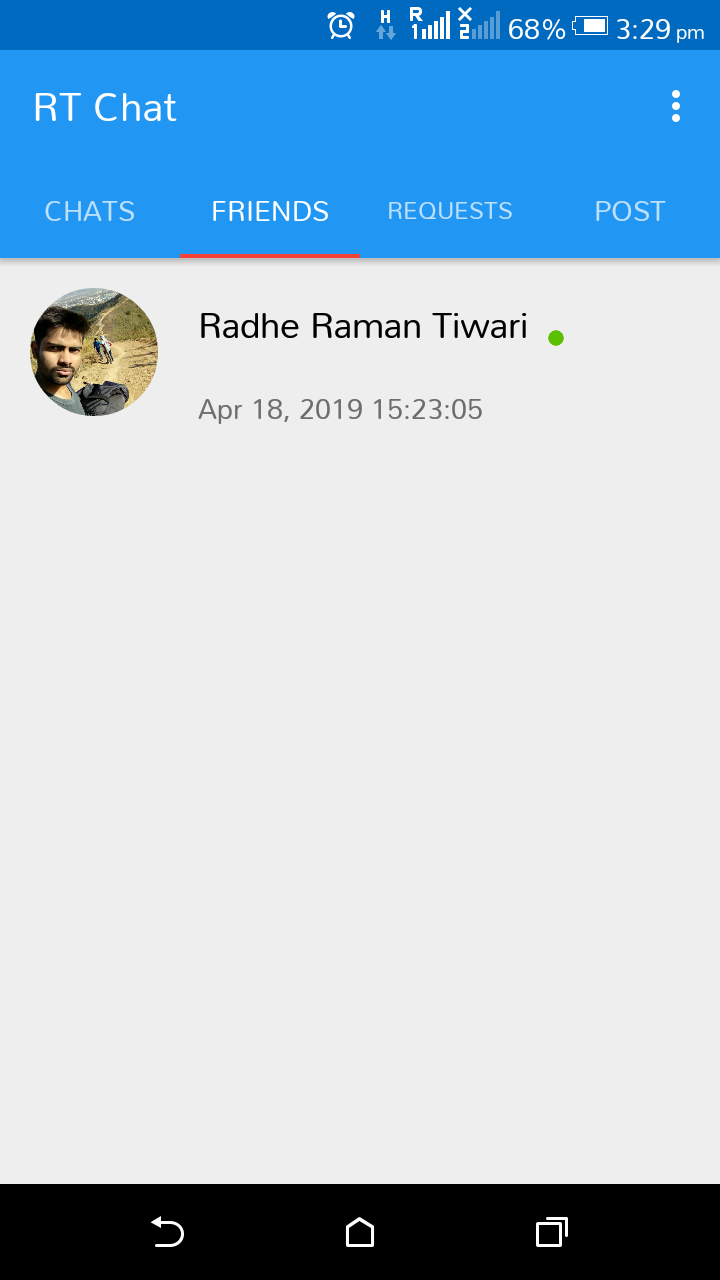
\includegraphics[scale=0.2]{home.png}
	\caption{\label{img15}  Home page activity contains four fragments.}
\end{figure}


\subsection{Test for Profile Page Activity}
There is following scenario come over user profile page activity...
\begin{itemize}
	\item It contains User profile image, user name, user status
	\item It also contains two button first button(i.e CHANGE IMAGE) for profile picture change and second button(i.e CHANGE STATUS) for user status change page activity.
\end{itemize}

\noindent
\begin{figure}[!ht]
	\centering
	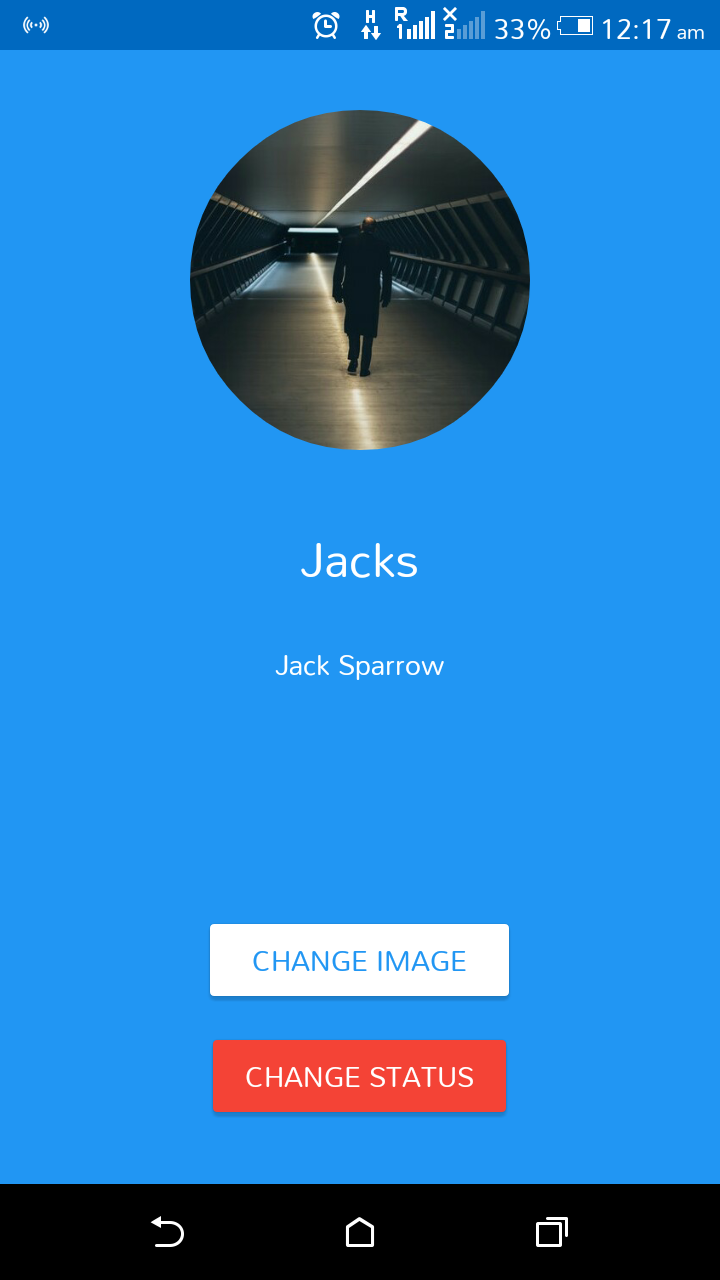
\includegraphics[scale=0.2]{profile-page.png}
	\caption{\label{img16}  User profile page activity.}
\end{figure}

\subsection{Test for Blog Post Page Activity}
There is following scenario come over blog post page activity...
\begin{itemize}
	\item It contains three fragments first Home, second Notification and third Account fragment.
	\item In Home fragment,user will see his and his friends blog post images and their description.
	\item In home fragment user can also like and commands to his or her and his or her friends blog posts.
	\item In blog post activity, there is one plus image when user clicks on it then it goes to new blog post activity where can add new blog image and their description.
	\item When user clicks on Account fragment then it goes to user profile.
\end{itemize}

\noindent
\begin{figure}[!ht]
	\centering
	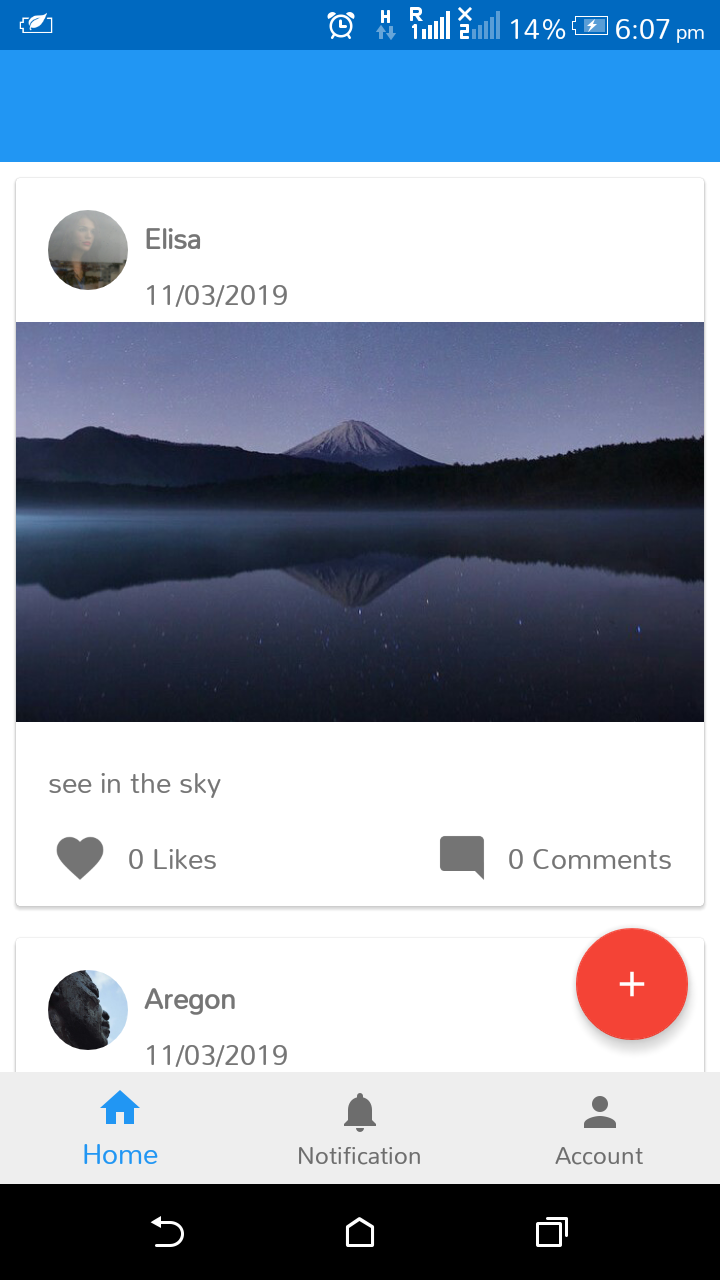
\includegraphics[scale=0.2]{blog-post.png}
	\caption{\label{img17} Blog post page activity.}
\end{figure}

\begin{figure}[!ht]
	\centering
	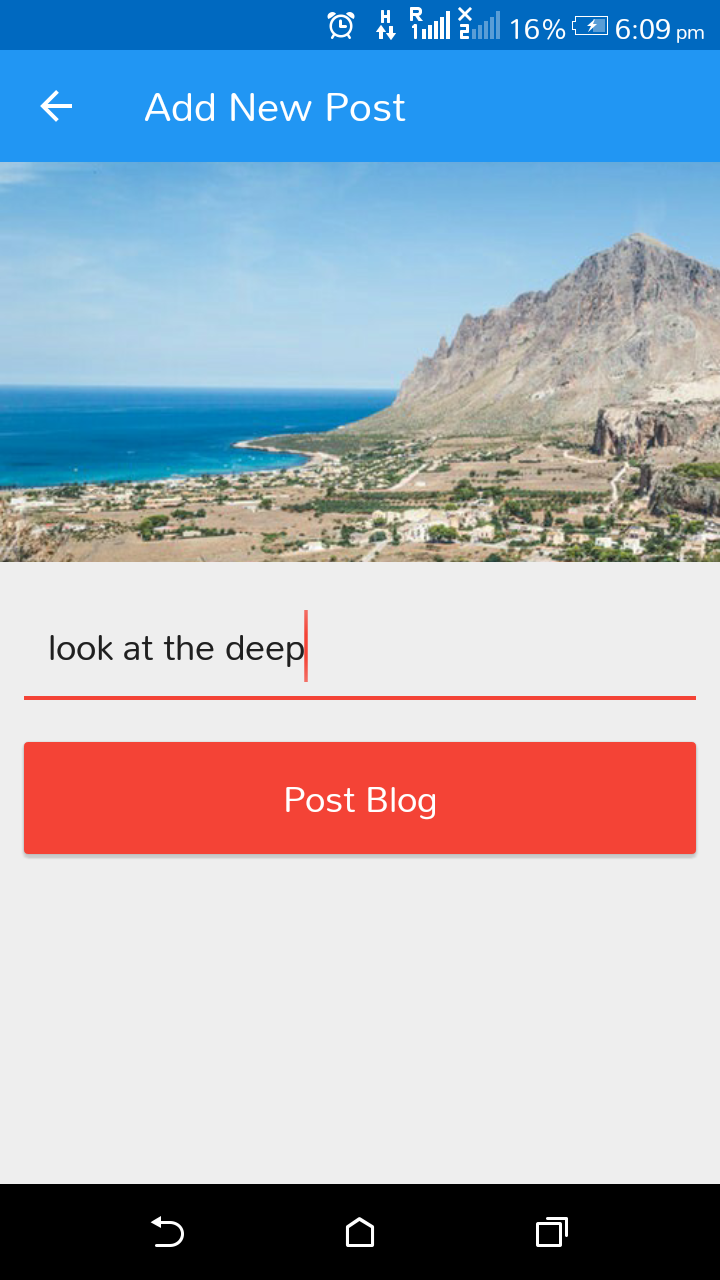
\includegraphics[scale=0.2]{new-post.png}
	\caption{\label{img17} New Post activity.}
\end{figure}





%+++++++++++++++++++++++++++++++++++++++++++++++++++++++++++++++++++++++++++++++++
%\section{Summary}
%\label{chap4:sum}
%In this chapter....

